%%%%%%%%%%%%%%%%%%%%%%%%%%%%%%%%%%%%%%%%%%%%%%%%%%%%%%%%%%%%%%%%%%%%%%%%%%%%%%%
% Copyright 2019
% Great Vespers, preceded by 9th Hour
%%%%%%%%%%%%%%%%%%%%%%%%%%%%%%%%%%%%%%%%%%%%%%%%%%%%%%%%%%%%%%%%%%%%%%%%%%%%%%%

\documentclass[twoside, letterpaper, 12pt]{report}
\usepackage{orthodoxservicebook}

\title{Great Vespers\\
Preceded by Ninth Hour}

\author{St. Katherine Orthodox Church}
\date{}% Remove date

\titlepic{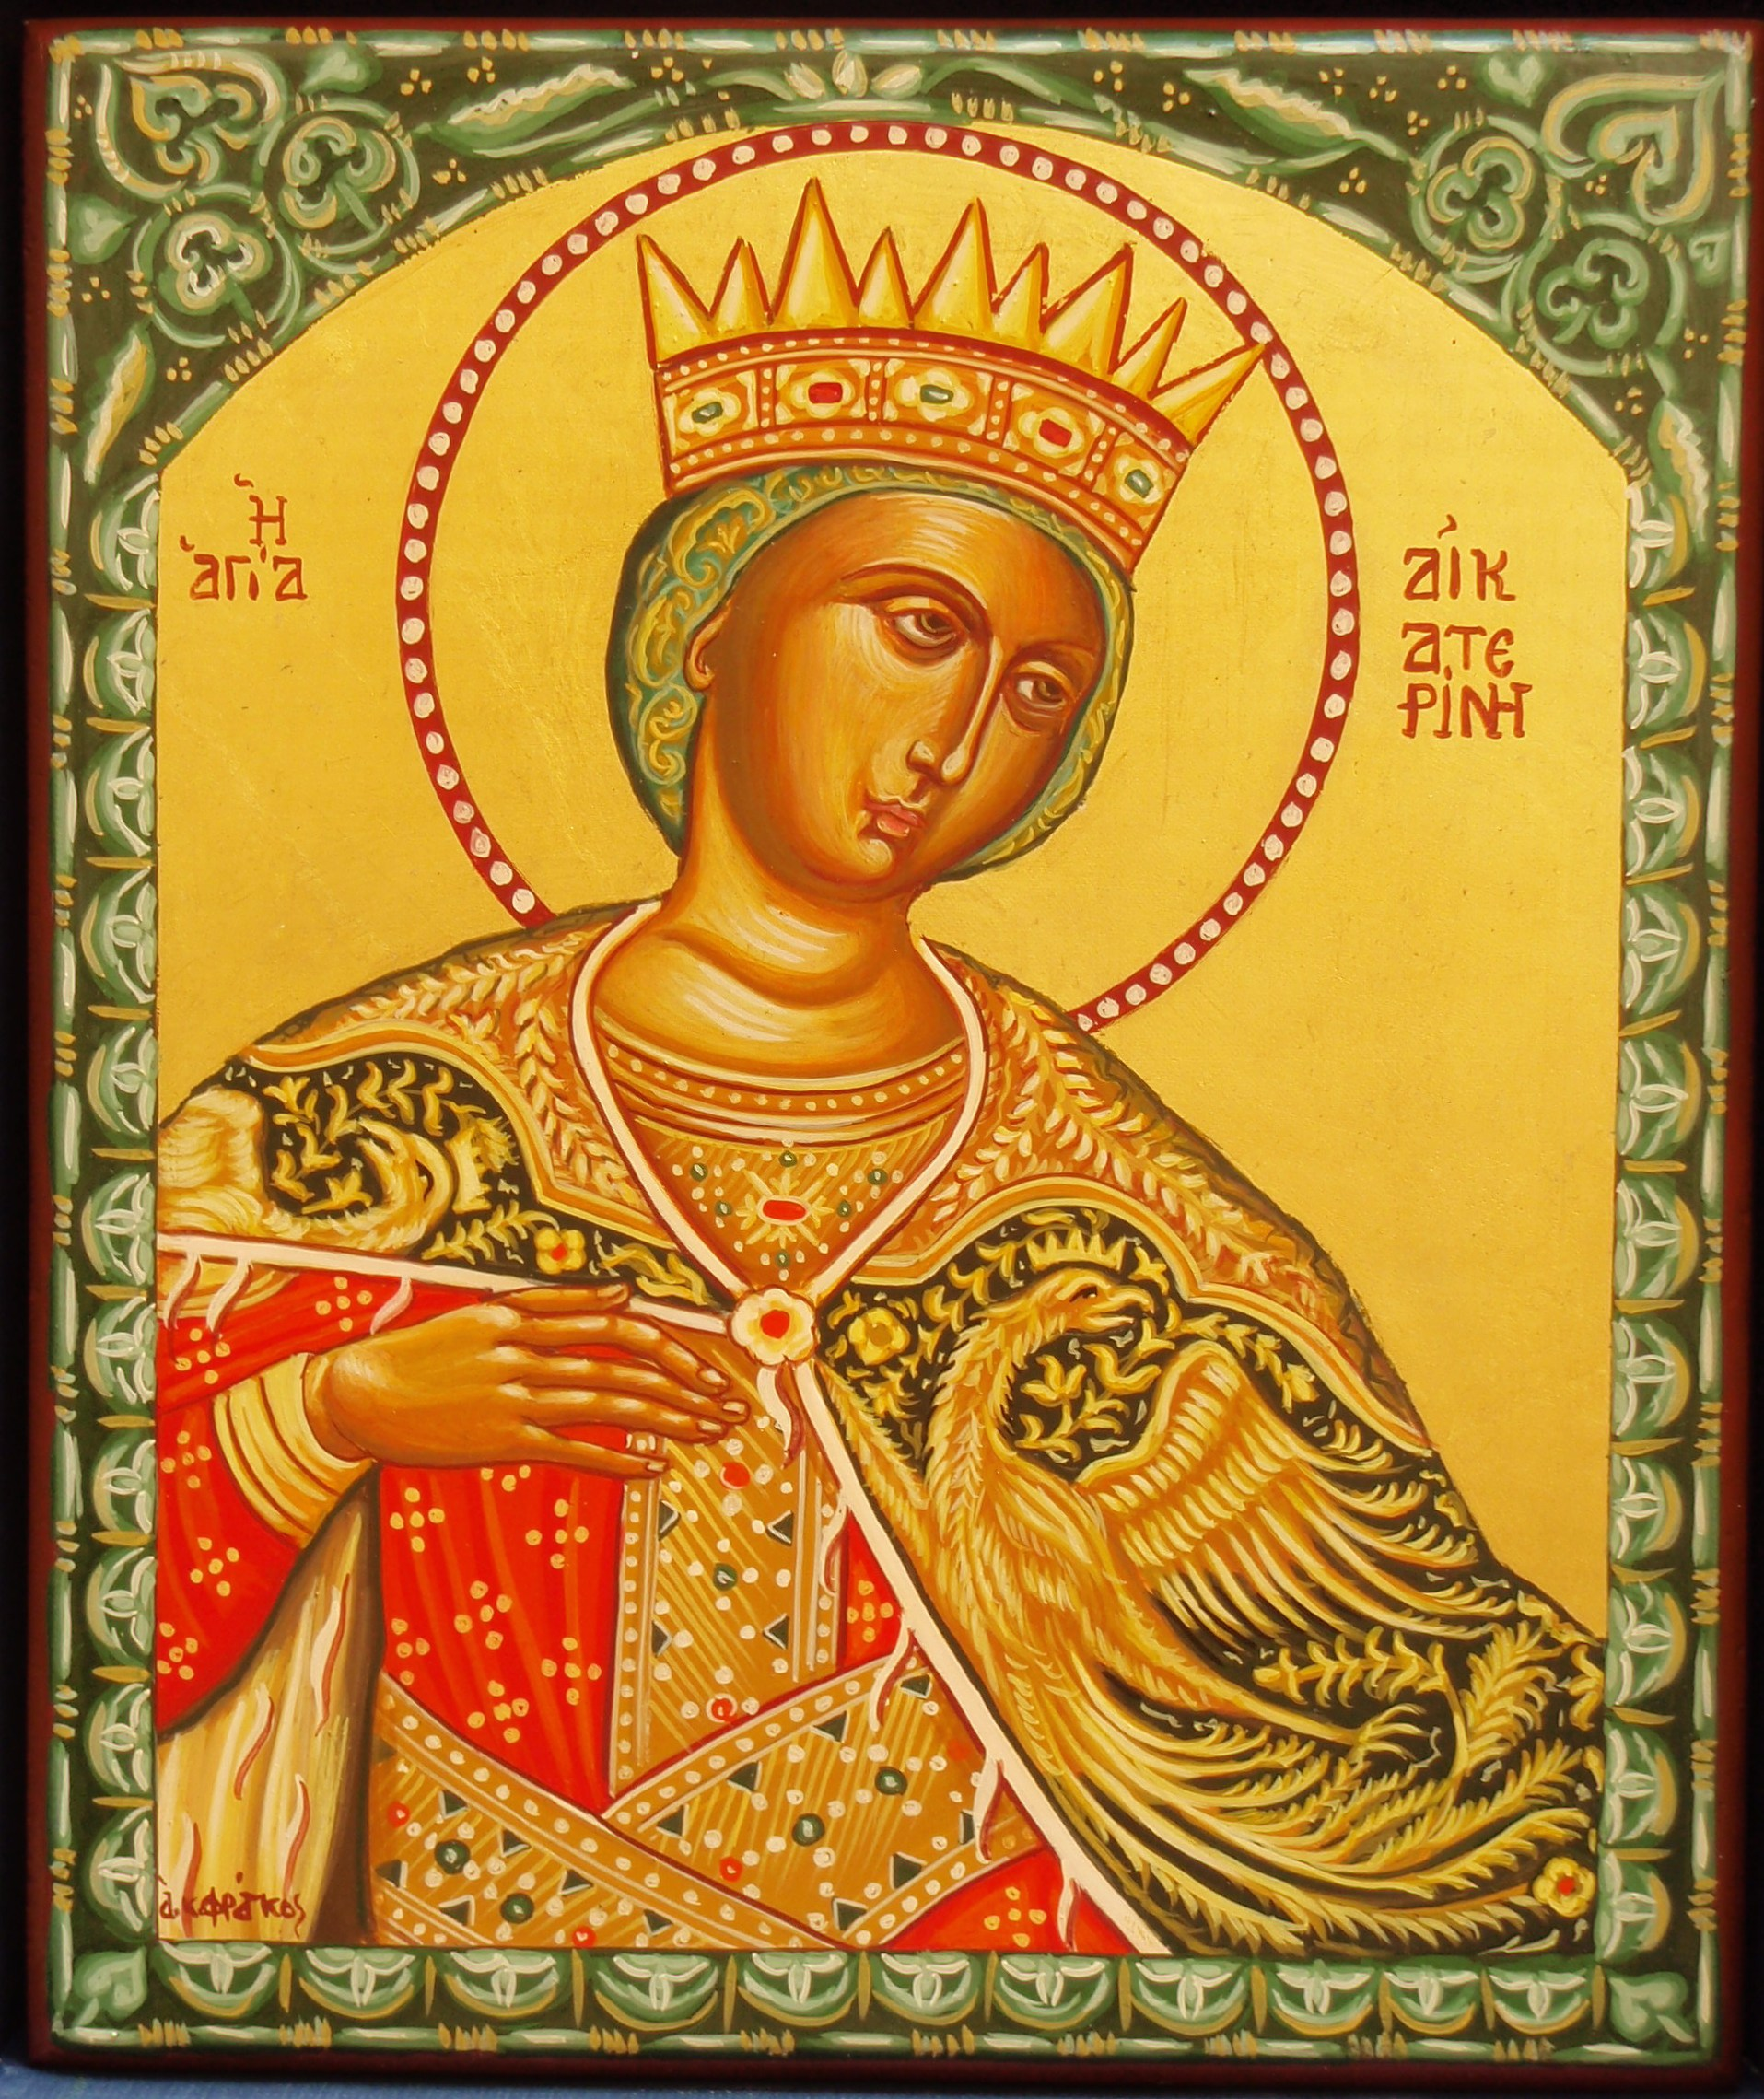
\includegraphics[width=0.5\textwidth]{Katherine1.jpg}}

\begin{document}
\maketitle
\pagestyle{empty} % Don't show page numbers

\instruction{This page intentionally left blank}

\cleardoublepage
\pagestyle{plain}
\setcounter{page}{1}
\chapter*{Ninth Hour}

% !TeX root = ../8-NinthHourSaturday.tex
%%%%%%%%%%%%%%%%%%%%%%%%%%%%%%%%%%%%%%%%%%%%%%%%%%%%%%%%%%%%%%%%%%%%%%%%%%%%%%%
% Copyright 2019
% This document contains the ninth hour prayers layout as LaTeX commands.
% This allows the command to me modified depending on the day provided
% as an argument, (FUTURE) inserting the appropriate psalms for the day.
%
% The closing content is provided as a separate command, so that it can
% be optionally included.
%
% The TEX commands in this document require the orthodoxservicebook.sty
%%%%%%%%%%%%%%%%%%%%%%%%%%%%%%%%%%%%%%%%%%%%%%%%%%%%%%%%%%%%%%%%%%%%%%%%%%%%%%%

\newcommand{\NinthHourContent}[1]{
\instruction{#1 - Plain Reading}
% TODO - Pull in the proper content based on the day of week argument

\priestline{Glory to Thee, O God \thrice}

\priestline{Blessed is our God always, now and ever, and unto ages of ages.}

\readerline{Amen.}

\instruction{Exclude from Pascha to Pentecost}
\begin{priest}
\item Glory to Thee, our God. Glory to Thee.
\item O heavenly King, Comforter, the Spirit of truth,
who art everywhere present and fillest all things,
the Treasury of good things and Giver of life:
Come and abide in us and cleanse us from every stain and save our souls,
O Good One.
\end{priest}

\instruction{From Pascha to Ascension - CHANT
\emph{``Christ is risen from the dead, trampling down death by death,
and upon those in the tombs, bestowing life.''}
(3x), and then SKIP the first line
\emph{``Holy God, Holy Mighty, Holy Immortal: have mercy on us. \thrice''}}

\centeredsection{The Trisagion Prayers}
\trisagionNeedsAmen{}

\begin{reader}
\item Amen.
\item Lord, have mercy. \twelve
\item Glory to the Father, and to the Son, and to the Holy Spirit;
  both now and ever, 
  and unto ages of ages. Amen.

\item O come, let us worship and fall down before God our King.\\
  O come, let us worship and fall down before Christ, our King and our God.\\
  O come, let us worship and fall down before the Very Christ, our King and our God.
\end{reader}
\begin{maybetwocolumns}
\squashedcenteredsection{Psalm 83} 
\input{./Psalms/Psalm083-unknwntrans.txt}

\squashedcenteredsection{Psalm 84}
\input{./Psalms/Psalm084-unknwntrans.txt}

\squashedcenteredsection{Psalm 85}
\input{./Psalms/Psalm085-unknwntrans.txt}

\needspace{2\baselineskip}
\instruction{And again:}

Work unto me a sign unto good, and let them that hate me behold and be put to shame;
for Thou, O Lord, hast holpen me and comforted me.

\end{maybetwocolumns}

\begin{reader}
  \item \gne
  \item Alleluia. Alleluia. Alleluia. Glory to Thee, O God. \thrice
  \item \lhmThree
  \item \glory
\end{reader}

\begin{maybetwocolumns}
\centeredsection{Apolytikion}
O ye apostles, martyrs and prophets, hierarchs,
venerable and righteous ones, who have 
finished well the contest and guarded the faith:
Beseech, we pray, since ye have boldness 
before the Savior who is good, that He may save our souls.

\readerline{\nowandever}

\centeredsection{Theotokion}

Thou who for our sake wast born of a virgin and didst suffer crucifixion,
O good One, 
and didst despoil death through death and as God didst reveal resurrection:
Despise not those whom Thou hast created with Thine own hand;
show forth Thy love for mankind,
O merciful One; accept the intercession of Thy mother, the Theotokos,
for us, and save Thy despairing people, O our Savior.

\vbox{}
Deliver us not up utterly, for Thy holy name’s sake,
neither disannul Thou Thy covenant, 
and cause not Thy mercy to depart from us,
for Abraham’s sake, Thy beloved,
and for Isaac’s sake, Thy servant,
and for Israel’s, Thy holy one.
\end{maybetwocolumns}

\centeredsection{Trisagion}
\trisagionNeedsAmen{}

\readerline{Amen.}

\begin{maybetwocolumns}
\instruction{Only one of the following:}

\centeredsection{(Not Lent) -- Kontakion}
\instruction{Outside of Lent}

Unto Thee, O Lord, the Author of creation, the universe doth offer the God-bearing
martyrs as the first-fruits of nature. By whose prayers, through the Theotokos,
do Thou preserve Thy Church in profound peace, O most merciful One.

\centeredsection{(Lent) -- Kontakion}
\instruction{During Lent}

When the thief beheld the Author of life hanging upon the cross, he said:
If Thou wert not God, who art here crucified with us,
then had the sun not veiled its rays,
neither would the earth have shaken with trembling.
But do Thou, who sufferest for all men, remember me,
O Lord, when Thou comest in Thy kingdom.

\vbox{}
Glory to the Father, and to the Son, and to the Holy Spirit.

\vbox{}
In the midst, between two thieves, was Thy cross found, the balance-beam of
righteousness; for while the one was led down to hades by the heaviness of his
blaspheming, the other was lightened of his sins,
unto the knowledge of things divine, O Christ God, glory to Thee.

\vbox{}
Both now and ever, and unto ages of ages. Amen.

\vbox{}
When she who bore Thee beheld upon the cross Thee, the Lamb and Shepherd and Savior
of the world, she weeping said: The world rejoiceth, in that it hath received redemption,
but my inward parts are inflamed as I behold Thy crucifixion, which Thou sufferest for all
men, O my Son and My God.

\centeredsection{Prayer of the Hours}
\readerline{\lhmForty}

Thou who, at all times and at every hour, both in heaven and on earth art
worshiped and glorified, O Christ God, long-suffering, plenteous in mercy
and compassion, who lovest the just and showest mercy to sinners, who callest
all men to salvation through the promise of good things to come: Do Thou, the
same Lord, receive also our supplications at this present hour, and direct our
lives according to Thy commandments. Sanctify our souls; purify our bodies;
set aright our minds; cleanse our thoughts; and deliver us from all calamity,
wrath and distress. Compass us round about with Thy holy Angels; that
guided and guarded by their hosts, we may attain unto the unity of the faith,
and unto the comprehension of Thine ineffable glory. For blessed art Thou unto
ages of ages. Amen.
\end{maybetwocolumns}

% if the end of maybetwocolumns is to close to the bottom,
% the below text may look like it's part of the first column instead of
% reverting back to full page.
\needspace{5\baselineskip}
\begin{reader}
\item \lhmThree
\item \gne
\item \morehonorablethanthetherubim
\item Bless, father in the name of the Lord.
\end{reader}

\priestline{May God have compassion upon us and bless us;
may He show the light of His countenance upon us and be merciful unto us.}

\readerline{Amen.}

\centeredsection{(Lent) -- The Prayer of Saint Ephraim the Syrian}
\instruction{During Lent}
\begin{priest}
\item O Lord and Master of my life,
    take from me the spirit of sloth, meddling, lust of power and idle talk.
    \instruction{prostration}
\item But give rather the spirit of chastity, humility,
    patience and love to thy servant.
    \instruction{prostration}
\item Yea, O Lord and King, grant me to see my own sins and not to judge my brother,
    for Thou art blessed unto ages of ages, Amen.
    \instruction{prostration}
\end{priest}

\instruction{Then, twelve metanias are made saying each time:}
\priestline{O God, be gracious unto me the sinner.}

\instruction{The prayer of Saint Ephraim is said again with only one prostration
  being made at the conclusion of it.}

\vbox{}
\trisagionNeedsAmen{}

\begin{reader}
\item Amen.
\item \lhmTwelve
\end{reader}

\centeredsection{Prayer of St. Basil the Great}
\begin{maybetwocolumns}
O Master, Lord Jesus Christ our God, who art long-suffering toward our sins
and who hast led us even to the present hour, in which, as Thou didst hang
upon the life-giving tree Thou didst make a way into paradise for the penitent
thief and by death didst destroy death: Be gracious unto us sinners and Thine
unworthy servants; for we have sinned and dealt iniquitously, and we are not
worthy to lift up our eyes and look upon the heights of heaven, inasmuch as
we have departed from the path of Thy righteousness and have walked after the
desires of our own hearts. But we implore of Thy boundless goodness: Spare
us, O Lord, according to the multitude of Thy mercy, and save us, for Thy holy
name’s sake; for our days have passed away in vanity. Wrest us out of the
hand of the adversary, and forgive our sins, and mortify our carnal
imagination, that, putting off the old man, we may be clothed upon with the
new man and may live unto Thee, our Master and our Benefactor, and that, so
following after Thy commandments, we may attain unto rest eternal, where is
the abode of all those who rejoice. For Thou art, in verity, the true Joy and
Exultation of those who love Thee, O Christ our God, and unto Thee we ascribe
glory, together with Thine unoriginate Father and Thine all-holy and good and
life-giving Spirit, now and ever, and unto ages of ages. Amen.
\end{maybetwocolumns}
}

\newcommand{\NinthHourClosingContent}{
% This is omitted when Vespers follows immediately.
\priestline{Glory to Thee, O Christ our God and our Hope, glory to Thee.}

\begin{reader}
\item Glory to the Father and to the Son and to the Holy Spirit,
  both now and ever, and unto ages of ages. Amen.
\item \lhmThree
\item Father, bless.
\end{reader}

\begin{priest}
\item May Christ our true God,
  through the intercessions of His all-immaculate and all-blameless holy Mother;
  of the holy, glorious, and right-victorious martyrs;
  of our venerable and God-bearing fathers; of the holy and righteous ancestors
  of God, Joachim and Anna; of (N., saint of the day), whose memory we
  celebrate and of all the saints: have mercy upon us, and save us,
  forasmuch as He is good and loveth mankind.
\item Through the prayers of our holy fathers, Lord Jesus Christ our God,
  have mercy on us, and save us.
\end{priest}

\readerline{Amen.}
}
 % Get all of the content
\NinthHourContent{Saturday}

\cleardoublepage
\chapter*{Great Vespers}
\begin{priest}
\item Blessed is our God, always, now and ever, and unto ages of ages.
\end{priest}

\choralresponse{./Z-Responses/HannonMinor/Amen.ly}

\begin{reader}
\item Come, let us worship and fall down before God our King.\\
    Come, let us worship and fall down before Christ, our King and our God.\\
    Come, let us worship and fall down before Christ Himself, our King and our God.\\
\end{reader}

\centeredsection{Psalm 103}
\begin{maybetwocolumns}
\input{Psalms/Psalm103.txt}

The sun knoweth his going down.
Thou appointedst the darkness, and there was the night.
How magnified are Thy works, O Lord! In wisdom hast Thou made them all.
\end{maybetwocolumns}

\lilypondfile{./Common/Alleluia-GloryToThee/Alleluia3x-GloryToTheex3x3OOurGod-Music.ly}

\centeredsection{The Great Litany}
\begin{maybetwocolumns}
\instruction{Repeat the responses, alternating between them, for each petition.}
\begin{deacon}
\item In peace, let us pray to the Lord.
\end{deacon}
\choralresponse{./Z-Responses/HannonMinor/LordHaveMercy-A.ly}

\begin{deacon}
\item For the peace from above, and for the salvation of our souls,
    let us pray to the Lord.
\end{deacon}
\choralresponse{./Z-Responses/HannonMinor/LordHaveMercy-B.ly}

\begin{deacon}
\item For the peace of the whole world, for the good estate of the Holy Churches of God,
    and for the union of all men, let us pray to the Lord.
\item For this Holy House, and for those who with faith, reverence, and fear of God,
    enter therein, let us pray to the Lord.
\item For our father and Metropolitan N., (for our Archbishop N. or Bishop N.),
    for the venerable Priesthood, the Diaconate in Christ,
    for all the clergy and the people, let us pray to the Lord.
\item  For the President of the United States, for all civil authorities,
    and for our Armed Forces everywhere, let us pray to the Lord.
\item For this city, and for every city and land, and for the faithful who dwell
    therein, let us pray to the Lord.
\item For healthful seasons, for abundance of the fruits of the earth,
    and for peaceful times, let us pray to the Lord.
\item For travelers by sea, by land, and by air; for the sick and the suffering;
    for captives and their salvation, let us pray to the Lord.
\item For our deliverance from all tribulation, wrath, danger, and necessity,
    let us pray to the Lord.
\item  Help us; save us; have mercy on us; and keep us, O God, by Thy grace.
\item Calling to remembrance our all-holy, immaculate, most blessed and glorious Lady Theotokos
    \instruction{(Recited quietly as the petitioner continues)}\\
    \lilypondfile[staffsize=16]{./Z-Responses/HannonMinor/MostHolyTheotokosSaveUs.ly}\\
    and ever-virgin Mary, with all the Saints: let us commend ourselves and
    each other, and all our life unto Christ our God.
\end{deacon}

\choralresponse{./Z-Responses/HannonMinor/ToTheeOLord.ly}

\begin{priest}
\item For unto Thee are due all glory, honor, and worship: to the Father,
    and to the Son, and to the Holy Spirit; now and ever and unto ages of ages.
\end{priest}

\choralresponse{./Z-Responses/HannonMinor/Amen.ly}
\end{maybetwocolumns}


\centeredsection{Psalm 140 - Lord I Have Cried}
\instruction{Chanted in the tone of the week. Insert Stanzas as prescribed.}

\vbox{}
\instruction{A doxasticon may be prescribed after the last stanza and
``Glory to the Father, Son and Holy Spirit''}

\vbox{}
\instruction{Finish with the Theotokion prescribed after ``Both now and ever..'',
which is generally the Theotokion of the Resurrection in the tone of the week.
}
\cleardoublepage

\centeredsection{The Holy Entrance}

\instruction{When the clergy reach the center of the solea,
the first part of the great censing begins. After the first part of the great
censing is completed, this next dialogue occurs quietly.}

\vbox{}
{
\footnotesize
Deacon: Bless, Father, the Holy Entrance.

Priest: Blessed is the entrance to Thy Holy Place, always, now and ever, and unto ages of ages. Amen.
}

\vbox{}
\instruction{After the choir has finished, the following is said aloud.}

\begin{deacon}
\item Wisdom! Let us attend!
\end{deacon}

\lilypondfile{./1-Vespers/Gladsome_Light/JoyousLightByz-Music.ly}

\centeredsection{Prokeimenon in the Tone of the Day}

\instruction{Tone 6 shown here is for Saturday Evening}

\begin{deacon}
    \item The Evening Prokeimenon!
\end{deacon}

\lilypondfile{./1-Vespers/Prokeimenon/Prokeimenon-AntiochianVillage-Tone6-SaturdayEvening-Music.ly}


\centeredsection{The Litany of Fervent Supplication}
\begin{maybetwocolumns}
\begin{deacon}
\item Let us say with our whole soul, and with our whole mind, let us say.
\end{deacon}
\choralresponse{./Z-Responses/HannonMinor/LordHaveMercy-A.ly}

\begin{deacon}
\item O Lord Almighty, the God of our Fathers, we pray Thee, hearken and have mercy.
\end{deacon}
\choralresponse{./Z-Responses/HannonMinor/LordHaveMercy-B.ly}

\begin{deacon}
\item Have mercy on us, O God, according to Thy great mercy, we pray Thee, hearken
    and have mercy.
\end{deacon}
\end{maybetwocolumns}
\instruction{Repeat the below response for each petition.}
\lilypondfile{./Z-Responses/HannonMinor/LordHaveMercyX3.ly}

\begin{maybetwocolumns}
\needspace{5\baselineskip}
\begin{deacon}
\item Again we pray for all pious and Orthodox Christians.
\item Again we pray for our father and Metropolitan N., (and for our Archbishop N. or Bishop N.).
\item Again we pray for our brethren: the priests, hieromonks, deacons, hierodeacons and monastics
    and all our brotherhood in Christ.
\item Again we pray for mercy, life, peace, health, salvation and visitation and pardon and
    remission of sins for (the servants of God, [Names], and) all Orthodox Christians of true
    worship, who live and dwell in this community.
\item Again we pray for the blessed and ever-memorable founders of this holy church and (for
    the departed servants of God, [Names], and) all our fathers and brethren, the Orthodox
    departed this life before us, who here and in all the world lie asleep in the Lord.
\item Again we pray for those who bear fruit and do good works in this holy and all venerable
    temple, those who serve and those who sing, and for all the people here present,
    who await Thy great and rich mercy.
\end{deacon}

\begin{priest}
\item For Thou art a merciful God and lovest mankind, and unto Thee we ascribe glory:
    to the Father, and to the Son, and to the Holy Spirit; now and ever, and unto ages of ages
\end{priest}

\choralresponse{./Z-Responses/HannonMinor/Amen.ly}
\end{maybetwocolumns}

\centeredsection{The Evening Prayer}
\instruction{Recited together as a congregation}

Vouchsafe, O Lord, to keep us this evening without sin.
Blessed art Thou, O Lord, the God of our fathers,
and praised and glorified is Thy Name forever. Amen.

Let Thy mercy be upon us, O Lord, even as we have set our hope on Thee.
Blessed art Thou, O Lord; teach me Thy statutes. Blessed art Thou, O Master;
make me to understand Thy statutes.
Blessed art Thou, O Holy One; enlighten me with Thy statutes.

Thy mercy, O Lord, endureth forever. O despise not the works of Thy hands.
To Thee belongeth worship, to Thee belongeth praise, to Thee belongeth glory:
to the Father, and to the Son, and to the Holy Spirit;
now and ever, and unto ages of ages. Amen.

\centeredsection{The Litany of Supplication}
\begin{maybetwocolumns}
\begin{deacon}
\item Let us complete our evening prayer unto the Lord.
\end{deacon}
\choralresponse{./Z-Responses/HannonMinor/LordHaveMercy-A.ly}

\begin{deacon}
\item Help us; save us; have mercy on us; and keep us, O God, by Thy grace.
\end{deacon}
\choralresponse{./Z-Responses/HannonMinor/LordHaveMercy-B.ly}

\needspace{10\baselineskip}
\begin{deacon}
\item That the whole evening may be perfect, holy, peaceful and sinless,
    let us ask of the Lord.
\end{deacon}
\instruction{Repeat these responses, alternating between them, for each remaining petition.}

\choralresponse{./Z-Responses/HannonMinor/GrantThisOLord-A.ly}

\begin{deacon}
\item An angel of peace, a faithful guide, a guardian of our souls and bodies,
    let us ask of the Lord.
\end{deacon}
\choralresponse{./Z-Responses/HannonMinor/GrantThisOLord-B.ly}

\begin{deacon}
\item Pardon and remission of our sins and transgressions, let us ask of the Lord.
\item All things good and profitable for our souls and peace for the world, let us ask of the Lord.
\item That we may complete the remaining time of our life in peace and repentance, let
    us ask of the Lord.
\item A Christian ending to our life, painless, blameless, peaceful, and a good defense
    before the fearful judgment seat of Christ, let us ask of the Lord.
\item Calling to remembrance our all-holy, immaculate, most blessed and glorious Lady Theotokos\\
    \instruction{(Recited quietly as the petitioner continues)}\\
    \lilypondfile[staffsize=16]{./Z-Responses/HannonMinor/MostHolyTheotokosSaveUs.ly}\\
    and ever-virgin Mary, with all the Saints: let us commend ourselves and each other,
    and all our life unto Christ our God.
\end{deacon}
\choralresponse{./Z-Responses/HannonMinor/ToTheeOLord.ly}

\begin{priest}
\item For Thou art a good God and lovest mankind, and unto Thee we ascribe glory:
    to the Father, and to the Son, and to the Holy Spirit; now and ever, and unto ages of ages.
\end{priest}

\choralresponse{./Z-Responses/HannonMinor/Amen.ly}
\end{maybetwocolumns}


\centeredsection{The Peace}
\begin{maybetwocolumns}
\begin{priest}
\item Peace be to all.
\end{priest}
\choralresponse{./Z-Responses/HannonMinor/AndToThySpirit.ly}

\begin{deacon}
\item Let us bow our heads unto the Lord.
\end{deacon}

\choralresponse{./Z-Responses/HannonMinor/ToTheeOLord.ly}

\instruction{All bow their heads as the priest says the following prayer:}
\begin{priest}
\item O Lord our God, Who didst bow the heavens and come down for the salvation of
    mankind: Look upon Thy servants and Thine inheritance; for unto Thee, the fearful
    Judge Who yet lovest mankind, have Thy servants bowed their heads and
    submissively inclined their necks, awaiting not help from men but entreating Thy
    mercy and looking confidently for Thy salvation. Guard them at all times, both
    during this present evening and in the approaching night, from every foe, from all
    adverse powers of the devil, and from vain thoughts and from evil imaginations.
\item Blessed and glorified be the might of Thy kingdom: of the Father, and of the Son,
    and of the Holy Spirit; now and ever, and unto ages of ages.
\end{priest}

\choralresponse{./Z-Responses/HannonMinor/Amen.ly}
\end{maybetwocolumns}


\centeredsection{Aposticha}
\instruction{Chanted in the tone of the week. Insert Stanzas as prescribed.}

\vbox{}
\instruction{A doxasticon may be prescribed after the last stanza and
``Glory to the Father, Son and Holy Spirit''}

\vbox{}
\instruction{Finish with the Theotokion prescribed after ``Both now and ever..'',
which is generally the Theotokion of the Resurrection in the tone of the doxasticon.
}

\cleardoublepage

\centeredsection{The Hymn of St. Simeon the God-receiver}
\instruction{Recited together as a congregation}

Lord, now lettest thou Thy servant depart in peace, according to Thy word; for mine eyes
have seen Thy salvation, which Thou hast prepared before the face of all people, a light to lighten
the Gentiles and the glory of Thy people Israel.

\centeredsection{The Trisagion Prayers}
\instruction{Recited together as a congregation}

Holy God, Holy Mighty, Holy Immortal: have mercy on us. \instruction{(THRICE)}

\vbox{}
\emph{Glory to the Father, and to the Son, and to the Holy Spirit; both now and ever, and
unto ages of ages. Amen.}

\vbox{}
All-holy Trinity, have mercy on us. Lord, cleanse us from our sins. Master, pardon
our iniquities. Holy God, visit and heal our infirmities for Thy Name’s sake.

\vbox{}
Lord, have mercy. \instruction{(3x)}

\vbox{}
\emph{Glory to the Father, and to the Son, and to the Holy Spirit; both now and ever, and
unto ages of ages. Amen.}

\vbox{}
Our Father, Who art in Heaven, hallowed be Thy Name. Thy kingdom come; Thy
will be done on earth as it is in Heaven. Give us this day our daily bread; and forgive
us our trespasses, as we forgive those who trespass against us, and lead us not into
temptation, but deliver us from evil.

\begin{priest}
\item For Thine is the kingdom, and the power, and the glory:
    of the Father, and of the Son, and of the Holy Spirit; now and ever, and unto ages of ages.
\end{priest}
\choralresponse{./Z-Responses/HannonMinor/Amen.ly}


\centeredsection{Apolytikion}
\instruction{Chanted in the tone of the week.}

\vbox{}
\instruction{Additional Apolytikion may be prescribed. Insert after
``Glory to the Father, Son and Holy Spirit''.}

\vbox{}
\instruction{Finish with the Theotokion prescribed after ``Both now and ever..'',
which is generally the Theotokion of the Resurrection in the tone of the last Apolytikion prescribed.
}

\centeredsection{The Dismissal}

\begin{deacon}
\item Wisdom!
\end{deacon}
\choralresponse{./Z-Responses/HannonMinor/FatherBless.ly}

\begin{priest}
\item Christ our God, the Existing One, is blessed, always, now and ever,
    and unto ages of ages
\end{priest}
\lilypondfile{./Z-Responses/HannonMinor/Amen-PreserveOGod-Amen.ly}

\begin{priest}
\item Most holy Theotokos, save us.
\end{priest}
\lilypondfile{Z-Responses/HannonMinor/MoreHonrableThanTheCherubim.ly}

\begin{priest}
\item Glory to Thee, O Christ our God and our Hope, glory to Thee.
\end{priest}
\lilypondfile{Z-Responses/HannonMinor/GNE-Amen.ly}
\lilypondfile{Z-Responses/HannonMinor/LordHaveMercyX3-FatherBless.ly}

\begin{priest}
\item May \instruction{-insert the appointed characteristic phrase-}, Christ our true God, through the intercessions of His
    all-immaculate and all-blameless holy Mother; by the might of the Precious and Life-giving Cross;
    by the protection of the honorable Bodiless Powers of Heaven;
    at the supplication of the honorable, glorious Prophet, Forerunner and Baptist John;
    of the holy, glorious and all-laudable apostles;
    of the holy, glorious and right-victorious Martyrs;
    of our venerable and God-bearing Fathers;
    of Saint Katherine, the patron and protector of this holy mission;
    of the holy and righteous ancestors of God, Joachim and Anna;
    \instruction{-Additional Saints for the day listed here-} whose memory we celebrate today,
    and of all the saints;
    have mercy on us and save us, forasmuch as He is good and loveth mankind.
\item Through the prayers of our Holy Fathers, Lord Jesus Christ our God,
    have mercy upon us and save us.
\end{priest}
\choralresponse{./Z-Responses/HannonMinor/Amen.ly}

\end{document}
